
\providecommand{\myrootdir}{..}
\documentclass[\myrootdir/main.tex]{subfiles}

\begin{document}
\chapter{Discussion}
\label{sec:discussion}

This chapter presents the answers to our research questions:
\begin{simplebox}{Research Questions}
\begin{itemize}
  \item[\textbf{RQ1:}] Which criteria influence the suitability of a chunk retrieval technique for CI build logs?
  \item[\textbf{RQ2:}] Under which conditions are PBE, CTS, and KWS suited to retrieve information from CI build logs?
  \item[\textbf{RQ2.1:}] How many examples do PBE, CTS, and KWS need to perform best?
  \item[\textbf{RQ2.2:}] How structurally similar do the examples for PBE, CTS and KWS need to be for the techniques to be applicable?
  \item[\textbf{RQ2.3:}] How accurate are the retrievals of PBE, CTS, and KWS?
\end{itemize}
\end{simplebox}

The first section discusses for PBE, CTS and KWS separately in which cases they perform best.
It details for which types of input build logs, available training examples and consumption of the retrieved output each technique is suited.
In the following section we discuss which of these criteria should influence the decision on a technique most.
Based on our empirical comparison, we present a decision tree between the three techniques we investigated.

\section{Interpretation of Study Results}
This section discusses the study results for each of the analyzed chunk retrieval techniques separately.
It gives recommendations on which kind of information chunk targets are best for each technique and for what kind of usage the output is suitable.

\subsection{Program Synthesis by Example (PBE)}
\paragraph{Configuration and Input}
Our study results show that chunk retrieval with PBE gives best results when the training examples are from one structural category.
This means it is suited to retrieve information chunks that always have the same surrounding structure.
To extract for example the reason a build failed, the log passage describing the failure would always have to be started and ended the same way.

When the training examples are of the same structure, one to three examples are enough input for PROSE to synthesize a regular expression program.
In our study, additional training examples did not improve the chunk retrieval.

\paragraph{Retrieval Output Usage}
If the program synthesis succeeds and applying the regular expression program yields an output, PBE shows a high precision and high recall.
The tool clearly identifies a failing program synthesis or no output from the program applied to a build log.
Therefore, if there is an output, the user can have high confidence it is the correct output.
This makes output from PBE chunk retrieval well suited for consumption of other software components.

\subsection{Common Text Similarity (CTS)}
\paragraph{Configuration and Input}
Chunk retrieval using CTS also yields better results the fewer structural categories are present in the training examples.
The number of training examples had no noticeable influence on the extraction quality in our study.
Information retrieval techniques like text similarity commonly learn on a higher number of examples than we used for our study.
Future work is needed to investigate how many examples yield improvements in the chunk retrieval over a single training example.

Extracting the average number of lines present in the training examples seems to give the best balance of precision and recall for CTS\@.

\paragraph{Retrieval Output Usage}
CTS has good precision and recall on average, though the quality of a chunk retrieval run is very hard to predict from the given result.
Therefore, retrieval output from CTS is suited to be read by a human.

\subsection{Keyword Search (KWS)}
\paragraph{Configuration and Input}
The number of structural categories in the training examples have little impact on the extraction quality of KWS\@.
This makes KWS a good technique if there is little prior knowledge on how the desired BLI is represented in the build log to be analyzed.
For the example of extracting the reason the build failed, KWS is best suited if a build can fail in various steps logged by different tools and no pre-categorization of where the build failed is available.

With at least two training examples KWS achieves good recall.

Retrieving the average number of lines present in the outputs of the training examples around every found keyword yields reasonable recall.
Selecting 1.5 times as many lines around every found keyword does improve the recall within our study but also increases the proportion of lines retrieved overall and therefore decreases precision.

\paragraph{Retrieval Output Usage}
Even though KWS has the highest recall of all three techniques, its precision is also the lowest.
The output of a chunk retrieval with KWS is well suited to be read by humans.

\section{Recommendations of Suitable Techniques}
% This section unifies our study results of the chunk retrieval techniques PBE, CTS and KWS\@.
% It recommends which technique to use depending on the available configuration and 
After discussing three chunk retrieval techniques separately we now want to unify out results into one recommendation scheme.
We present a decision tree, which asks questions to a developer or researcher who wants to retrieve information chunks from build logs.
The answers lead the user to more questions or the recommended technique as leaf nodes.
Figure~\ref{fig:crt-recommendation} presents the decision tree.

\emph{Caveat!} This is a preliminary theory based on the results from our comparison study.
The recommendations are therefore likely based on our implementation of the chunk retrieval techniques as well as the logs in the \emph{LogChunks} data set.
This decision tree is the answer to our first research question about which criteria influence the suitability of a chunk retrieval technique.
The earlier in the decision tree a criterion is noted, the more important it is when distinguishing the techniques.

The first and most important aspect are the structural categories.
Are the information chunks you would like to retrieve always presented in the same structural way within the build logs?
Then the information chunks in all training examples and the analyzed build log are in the same structural category.

If the information chunks are from multiple structural categories, meaning the are not represented in the same structural way within the build logs, and recall is more important than precision we recommend to use KWS\@.
If the representations are from multiple structural categories and precision is more important than recall to the user we recommend CTS\@.
We also recommend CTS when the representations are from one structural category, the user does not require a high confidence in the accuracy of the outcome and the user rather have output with low recall instead of no output at all.
When the representations are from one structural category and the user wishes a high confidence in the correctness of the output or prefers no output over output with low recall, we recommend PBE\@.

\begin{table}[htbp]
\centering
\begin{tabularx}{\textwidth}{@{}llll@{}}
  \toprule
  & PBE & CTS & KWS \\
  \midrule
  Structural Categories & 1 & less is better & no influence \\
  Training Set Size & 1 - 3 & no influence & > 2 \\ 
  Precision & \makecell[l]{high \\ (if synthesis succeeds)} & medium & low \\ 
  Recall & \makecell[l]{high \\ (if synthesis succeeds)} & medium & high \\ 
  \makecell[l]{Confidence in \\ Output Correctness} & high & low & \makecell[l]{low (precision) \\ high (recall)} \\ 
  Output Consumption by & program & human & human \\ 
  \bottomrule
\end{tabularx}
\caption{Recommendations for each of the investigated chunk retrieval techniques}
\label{tab:single-technique-recommendations}
\end{table}

\begin{figure}[htbp]
		\centering
		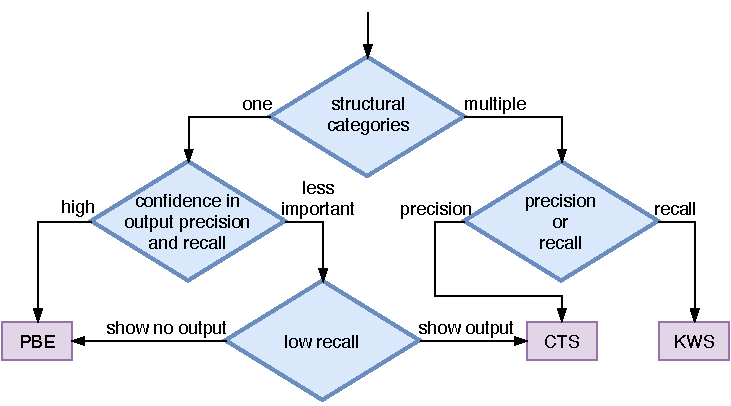
\includegraphics[width=\textwidth, clip]{img/crt-recommendation.pdf}
		\caption{Our preliminary recommendation scheme for chunk retrieval techniques}
		\label{fig:crt-recommendation}
\end{figure}

\section{Threats to Validity}

There are several threats to the validity of the conclusions of our work.

\paragraph{Implementation}
Our results are highly dependent on our implementation of the investigated chunk retrieval techniques and the libraries we used.
Our implementation of PBE is mainly based on the program synthesis provided by PROSE\@.
Its limitations are therefore also mainly influenced by this library.
For example, the need for examples from a single structural category stems from the fact that FlashExtract cannot learn regular expression programs with arbitrary boolean conjunctions and disjunctions~\cite{mayer2015user}.
This limitation was necessary to keep the synthesis performance reasonable.

Our implementation of CTS is dependent on the library tex2vec and the way they split strings into word tokens.
We intentionally chose a simple, minimally configured and tuned approach to compare against.
Tuning the text similarity meta-parameters more to the specific use case of chunk retrieval from build logs would yield better chunk retrieval results.

\paragraph{Data Set}
The outcomes of our comparison study are highly dependent on the build logs from the \emph{LogChunks} data set.
It only consists of build logs from open source and therefore it is not clear whether our results are generalizable to industry projects.
We only collected build logs from Travis CI, however we chose to evaluate on an information chunk whose format is not dependent on Travis CI\@.
This is because the reason the build failed is described within the build logs by the tools themselves and not the Travis CI environment.

\paragraph{Training Set Size}
Especially the results for CTS might influenced by the fact that we only trained on one to five examples.
We chose this small training set size as the training examples have to be provided per repository and we expect a developer to not want to provide more examples than the small numbers we evaluated on.

\paragraph{Few Samples with Many Structural Categories}
Our comparison study shows fewer measurements with many structural categories than with one category.
This stems from the fact that we use such a realistic data set which in many cases has only one or few structural categories.
% \bp{
% chronologically selected examples -> very specific view, devs/users might pick more representative examples

% very few evaluation runs with a high number of categories in configuring I/O examples -> because we chose to create such a ``realistic'' data set, from data set we see that many structural categories uncommon

% some errors are not shown inside the log: we always choose an extraction, if we did not see the actual reason for the error reported, we chose the part stating that an error occured / the build failed}
\end{document}
